\documentclass[UTF8,11pt]{ctexart}
\usepackage[a4paper,margin=22mm]{geometry}
\usepackage{amsmath,amssymb,bm,graphicx,adjustbox,fvextra,longtable,array}
\xeCJKDeclareCharClass{CJK}{"2160 -> "217F, "2460 -> "249B, "2200 -> "22FF}
\newcommand{\fitmath}[1]{\begin{adjustbox}{max width=\linewidth}$\displaystyle #1$\end{adjustbox}}
\setlength{\parindent}{0pt}\setlength{\parskip}{.65em}\renewcommand{\arraystretch}{1.3}
\sloppy\allowdisplaybreaks
\begin{document}
\section*{2024 年计算机统考 408 · 真题}
\subsection*{2024年全国硕士研究生入学统一考试}

\subsection*{计算机学科专业基础综合试题}

\subsection*{一、单项选择题（1～40小题，每小题2分，共80分。下列每小题给出的四个选项中，只有一项符合题目要求）}

1．已知带头结点的非空单链表L的头指针为h，结点结构为：


\begin{center}\begin{adjustbox}{max width=\linewidth}\begin{tabular}{|>{\raggedright\arraybackslash}p{\dimexpr(\linewidth-4\tabcolsep-3\arrayrulewidth)/2\relax}|>{\raggedright\arraybackslash}p{\dimexpr(\linewidth-4\tabcolsep-3\arrayrulewidth)/2\relax}|}\hline
data & next\\\hline\end{tabular}\end{adjustbox}\end{center}

其中next是指向直接后继结点的指针。现有指针p和q，若p指向L中非首且非尾的任意一个结点，则执行语句序列“q=p->next; p->next=q->next; q->next=h->next; h->next=q;”的结果是\_\_\_\_\_\_。


\begin{center}\begin{tabular}{>{\raggedright\arraybackslash}p{\dimexpr(\linewidth-4\tabcolsep)/2\relax}>{\raggedright\arraybackslash}p{\dimexpr(\linewidth-4\tabcolsep)/2\relax}}
\textbf{A.} 在p所指结点后插入q所指结点 & \textbf{B.} 在q所指结点后插入p所指结点\\[.35em]
\textbf{C.} 将p所指结点移动到L的头结点之后 & \textbf{D.} 将q所指结点移动到L的头结点之后\\[.35em]\end{tabular}\end{center}

2．表达式 \(\displaystyle x+y*(z-u)/v\) 的等价后缀表达式是\_\_\_\_\_\_。


\begin{center}\begin{tabular}{>{\raggedright\arraybackslash}p{\dimexpr(\linewidth-8\tabcolsep)/4\relax}>{\raggedright\arraybackslash}p{\dimexpr(\linewidth-8\tabcolsep)/4\relax}>{\raggedright\arraybackslash}p{\dimexpr(\linewidth-8\tabcolsep)/4\relax}>{\raggedright\arraybackslash}p{\dimexpr(\linewidth-8\tabcolsep)/4\relax}}
\textbf{A.} xyzu-*v/+ & \textbf{B.} xyzu-v/*+ & \textbf{C.} +x/*y-zuv & \textbf{D.} +x*y/-zuv\\[.35em]\end{tabular}\end{center}

3．p、q 和v 都是二叉树T 中的结点，v 有两个孩子结点，T 的中序遍历序列形如：“…, p, v, q, …”， 则下列叙述中，正确的是\_\_\_\_\_\_。


\begin{center}\begin{tabular}{>{\raggedright\arraybackslash}p{\dimexpr(\linewidth-4\tabcolsep)/2\relax}>{\raggedright\arraybackslash}p{\dimexpr(\linewidth-4\tabcolsep)/2\relax}}
\textbf{A.} p 没有右孩子，q 没有左孩子 & \textbf{B.} p 没有右孩子，q 有左孩子\\[.35em]
\textbf{C.} p 有右孩子，q 没有左孩子 & \textbf{D.} p 有右孩子，q 有左孩子\\[.35em]\end{tabular}\end{center}

4．给定无向图G = (V, E)的邻接多重表如下图所示，则G 中顶点b 与d 的度分别是


\begin{center}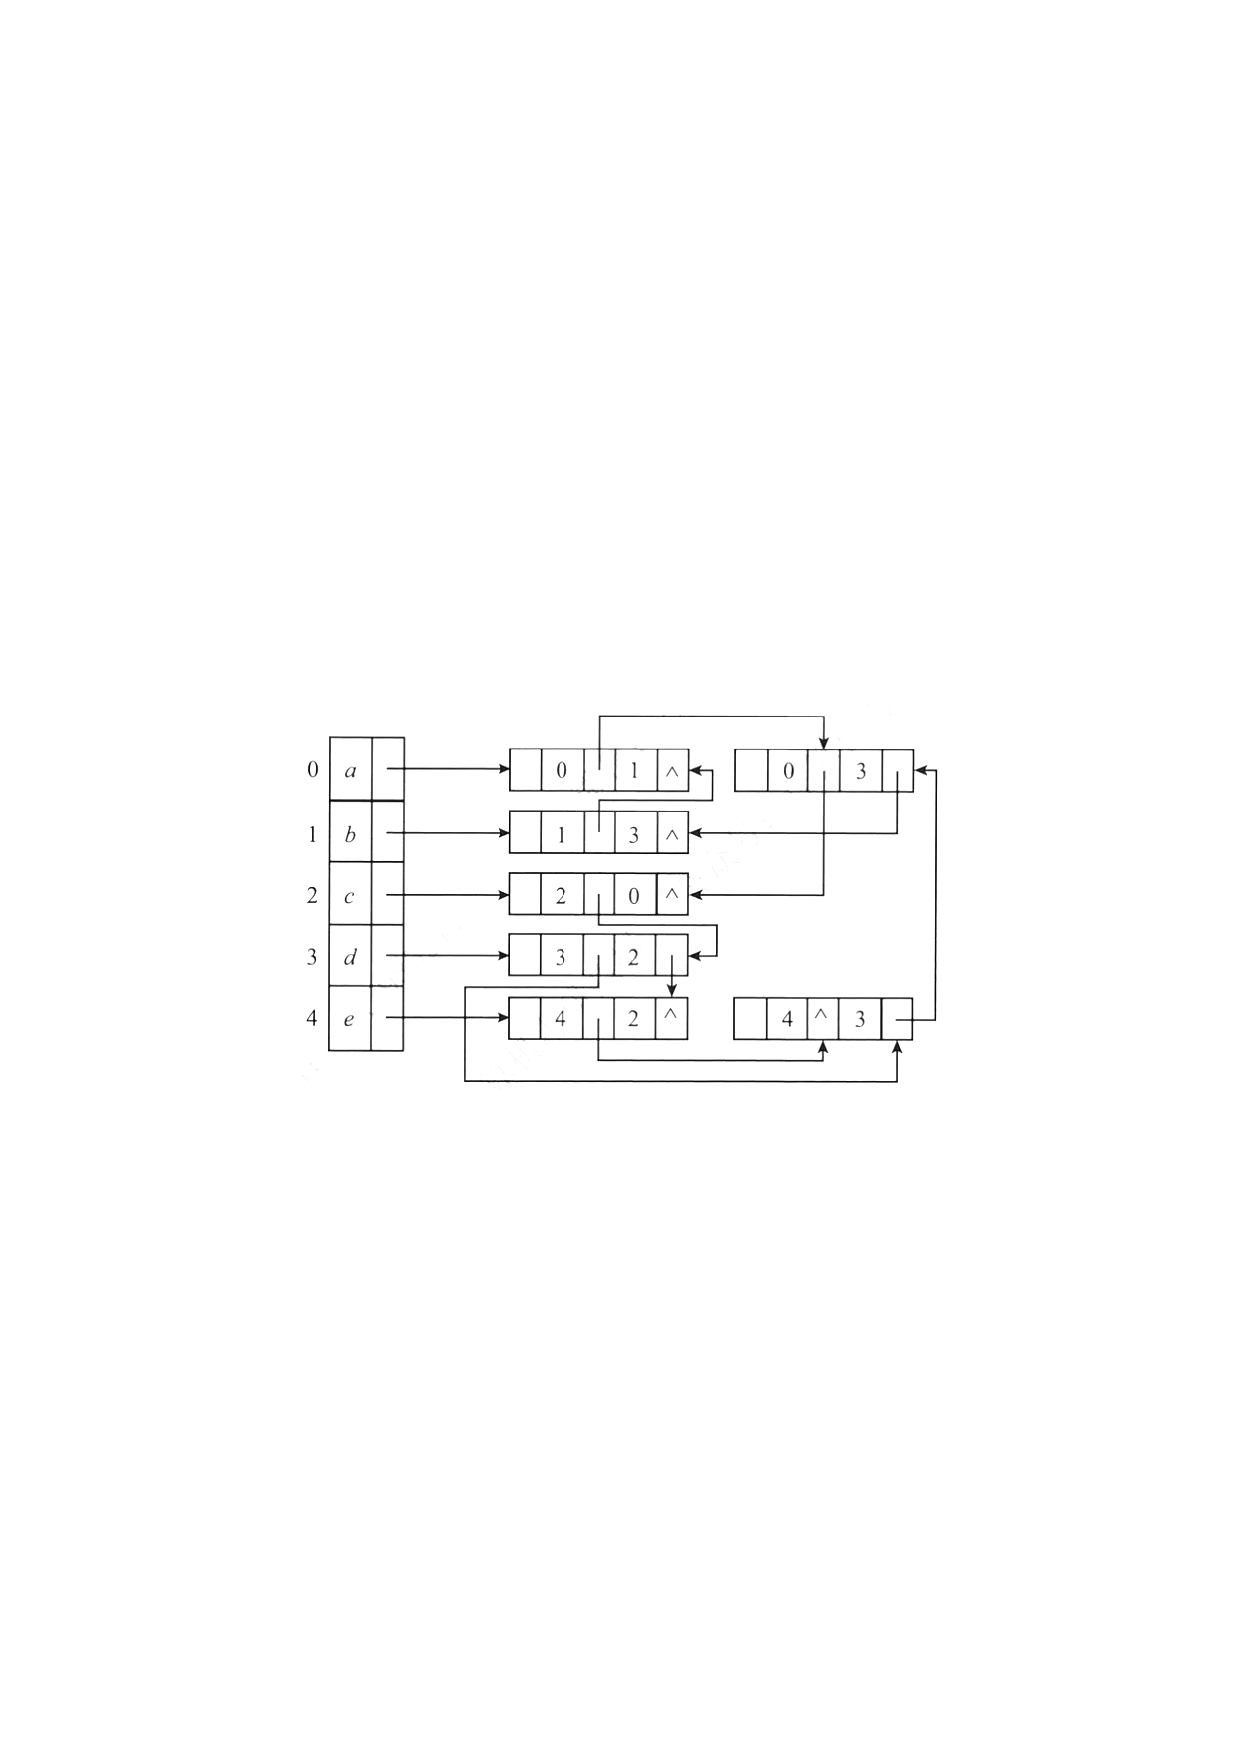
\includegraphics[width=.65\linewidth,height=.4\textheight,keepaspectratio]{../assets/figures/2024-questions-p001-b009.pdf}\end{center}

\begin{center}\begin{tabular}{>{\raggedright\arraybackslash}p{\dimexpr(\linewidth-8\tabcolsep)/4\relax}>{\raggedright\arraybackslash}p{\dimexpr(\linewidth-8\tabcolsep)/4\relax}>{\raggedright\arraybackslash}p{\dimexpr(\linewidth-8\tabcolsep)/4\relax}>{\raggedright\arraybackslash}p{\dimexpr(\linewidth-8\tabcolsep)/4\relax}}
\textbf{A.} 0, 2 & \textbf{B.} 2, 4 & \textbf{C.} 2, 5 & \textbf{D.} 3, 4\\[.35em]\end{tabular}\end{center}

5．下列数据结构中，不适合．．．直接使用折半查找的是\_\_\_\_\_\_。 I. 有序链表 II. 无序数组 III. 有序静态链表 IV. 无序静态链表


\begin{center}\begin{tabular}{>{\raggedright\arraybackslash}p{\dimexpr(\linewidth-8\tabcolsep)/4\relax}>{\raggedright\arraybackslash}p{\dimexpr(\linewidth-8\tabcolsep)/4\relax}>{\raggedright\arraybackslash}p{\dimexpr(\linewidth-8\tabcolsep)/4\relax}>{\raggedright\arraybackslash}p{\dimexpr(\linewidth-8\tabcolsep)/4\relax}}
\textbf{A.} 仅I、III & \textbf{B.} 仅II、IV & \textbf{C.} 仅II、III、IV & \textbf{D.} I、II、III、IV\\[.35em]\end{tabular}\end{center}

6．KMP 算法使用修正后的next 数组进行模式匹配，模式串S=“aabaab”，当主串中某字符与S 中某字符失配时，S 将向右滑动的最长距离是\_\_\_\_\_\_。


\begin{center}\begin{tabular}{>{\raggedright\arraybackslash}p{\dimexpr(\linewidth-8\tabcolsep)/4\relax}>{\raggedright\arraybackslash}p{\dimexpr(\linewidth-8\tabcolsep)/4\relax}>{\raggedright\arraybackslash}p{\dimexpr(\linewidth-8\tabcolsep)/4\relax}>{\raggedright\arraybackslash}p{\dimexpr(\linewidth-8\tabcolsep)/4\relax}}
\textbf{A.} 5 & \textbf{B.} 4 & \textbf{C.} 3 & \textbf{D.} 2\\[.35em]\end{tabular}\end{center}

7．一棵二叉搜索树如题7 图所示，\(\displaystyle k_1\)、\(\displaystyle k_2\)、\(\displaystyle k_3\) 分别是对应结点中保存的关键字。子树T 的任一结点中保存的关键字x 满足的是\_\_\_\_\_\_。 题7 图


\begin{center}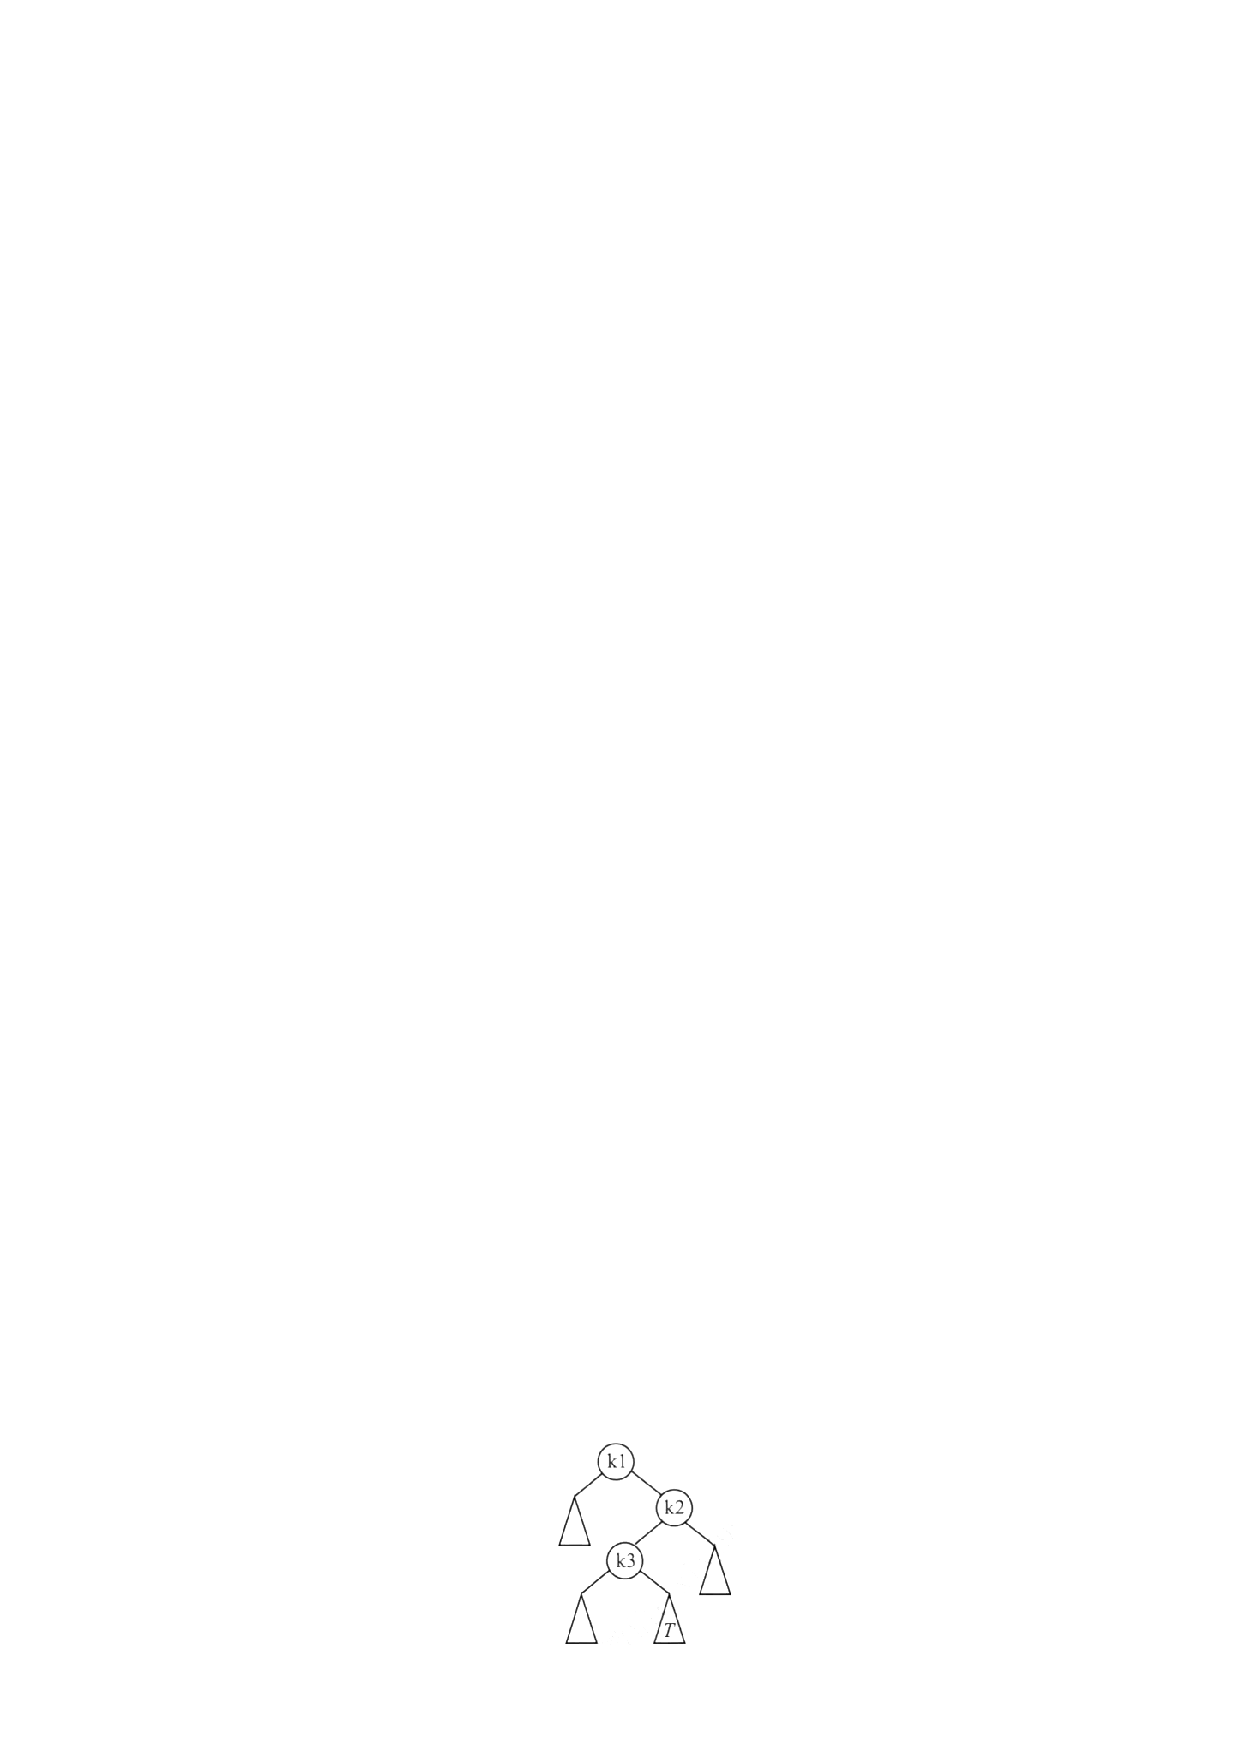
\includegraphics[width=.65\linewidth,height=.4\textheight,keepaspectratio]{../assets/figures/2024-questions-p001-b014.pdf}\end{center}

第7题（续）：


\begin{center}\begin{tabular}{>{\raggedright\arraybackslash}p{\dimexpr(\linewidth-4\tabcolsep)/2\relax}>{\raggedright\arraybackslash}p{\dimexpr(\linewidth-4\tabcolsep)/2\relax}}
\textbf{A.} x < \(\displaystyle k_1\) & \textbf{B.} x > \(\displaystyle k_2\)\\[.35em]
\textbf{C.} \(\displaystyle k_1\) < x < \(\displaystyle k_3\) & \textbf{D.} \(\displaystyle k_3\) < x < \(\displaystyle k_2\)\\[.35em]\end{tabular}\end{center}

8．使用快速排序算法对含n（n≥3）个元素的数组M 进行排序，若第一趟排序将M 中除枢轴外的n– 1 个元素划分为均不为空的P 和Q 两块，则下列叙述中，正确的是\_\_\_\_\_\_。


\begin{center}\begin{tabular}{>{\raggedright\arraybackslash}p{\dimexpr(\linewidth-4\tabcolsep)/2\relax}>{\raggedright\arraybackslash}p{\dimexpr(\linewidth-4\tabcolsep)/2\relax}}
\textbf{A.} P 和Q 块间有序 & \textbf{B.} P 和Q 均块内有序\\[.35em]
\textbf{C.} P 和Q 的元素个数大致相等 & \textbf{D.} P 中和Q 中均不存在相等的元素\\[.35em]\end{tabular}\end{center}

9．已知关键字序列28, 22, 20, 19, 8, 12, 15, 5 是大根堆（最大堆），对该堆进行两次删除操作后，得到的新堆是\_\_\_\_\_\_。


\begin{center}\begin{tabular}{>{\raggedright\arraybackslash}p{\dimexpr(\linewidth-4\tabcolsep)/2\relax}>{\raggedright\arraybackslash}p{\dimexpr(\linewidth-4\tabcolsep)/2\relax}}
\textbf{A.} 20, 19, 15, 12, 8, 5 & \textbf{B.} 20, 19, 15, 5, 8, 12\\[.35em]
\textbf{C.} 20, 19, 12, 15, 8, 5 & \textbf{D.} 20, 19, 8, 12, 15, 5\\[.35em]\end{tabular}\end{center}

10．现有由关键字组成的3 个有序序列(3，5)、(7，9)和(6)，若按从左至右的次序选择有序序列进行二路归并排序，则关键字之间的总比较次数是\_\_\_\_\_\_。


\begin{center}\begin{tabular}{>{\raggedright\arraybackslash}p{\dimexpr(\linewidth-8\tabcolsep)/4\relax}>{\raggedright\arraybackslash}p{\dimexpr(\linewidth-8\tabcolsep)/4\relax}>{\raggedright\arraybackslash}p{\dimexpr(\linewidth-8\tabcolsep)/4\relax}>{\raggedright\arraybackslash}p{\dimexpr(\linewidth-8\tabcolsep)/4\relax}}
\textbf{A.} 3 & \textbf{B.} 4 & \textbf{C.} 5 & \textbf{D.} 6\\[.35em]\end{tabular}\end{center}

11．在外排序中，利用败者树对初始为升序的归并段进行多路归并，败者树中记录“冠军”的结点保存的是\_\_\_\_\_\_。


\begin{center}\begin{tabular}{>{\raggedright\arraybackslash}p{\dimexpr(\linewidth-4\tabcolsep)/2\relax}>{\raggedright\arraybackslash}p{\dimexpr(\linewidth-4\tabcolsep)/2\relax}}
\textbf{A.} 最大关键字 & \textbf{B.} 最小关键字\\[.35em]
\textbf{C.} 最大关键字所在的归并段号 & \textbf{D.} 最小关键字所在的归并段号\\[.35em]\end{tabular}\end{center}

12．C语言代码如下：


\begin{Verbatim}[breaklines,breakanywhere,fontsize=\small]
int i = 32777;
short si = i;
int j = si;
\end{Verbatim}

执行上述代码段后，j的值是\_\_\_\_\_\_。


\begin{center}\begin{tabular}{>{\raggedright\arraybackslash}p{\dimexpr(\linewidth-8\tabcolsep)/4\relax}>{\raggedright\arraybackslash}p{\dimexpr(\linewidth-8\tabcolsep)/4\relax}>{\raggedright\arraybackslash}p{\dimexpr(\linewidth-8\tabcolsep)/4\relax}>{\raggedright\arraybackslash}p{\dimexpr(\linewidth-8\tabcolsep)/4\relax}}
\textbf{A.} －32 777 & \textbf{B.} －32 759 & \textbf{C.} 32 759 & \textbf{D.} 32 777\\[.35em]\end{tabular}\end{center}

13．通常情况下，将汇编语言程序中实现特定功能的指令序列定义成一条伪指令（pseudoinstruction）。 下列选项中，CPU 能理解并直接执行的是\_\_\_\_\_\_。 I. 伪指令 II. 微指令 III. 机器指令 IV. 汇编指令


\begin{center}\begin{tabular}{>{\raggedright\arraybackslash}p{\dimexpr(\linewidth-8\tabcolsep)/4\relax}>{\raggedright\arraybackslash}p{\dimexpr(\linewidth-8\tabcolsep)/4\relax}>{\raggedright\arraybackslash}p{\dimexpr(\linewidth-8\tabcolsep)/4\relax}>{\raggedright\arraybackslash}p{\dimexpr(\linewidth-8\tabcolsep)/4\relax}}
\textbf{A.} 仅I 和IV & \textbf{B.} 仅II 和III & \textbf{C.} 仅III 和IV & \textbf{D.} 仅I、II 和IV\\[.35em]\end{tabular}\end{center}

14．某科学实验中，需要使用大量的整型参数，为了在保证表数精度的基础上提高运算速度，需要选择合理的数据表示方法。若整型参数\(\displaystyle \alpha\)、\(\displaystyle \beta\)的取值范围分别为\(\displaystyle -2^{20}\sim2^{20}\)、\(\displaystyle -2^{40}\sim2^{40}\)，则下列选项中，\(\displaystyle \alpha\)、\(\displaystyle \beta\)最适宜采用的数据表示方法分别是\_\_\_\_\_\_。


\begin{center}\begin{tabular}{>{\raggedright\arraybackslash}p{\dimexpr(\linewidth-4\tabcolsep)/2\relax}>{\raggedright\arraybackslash}p{\dimexpr(\linewidth-4\tabcolsep)/2\relax}}
\textbf{A.} 32位整数、32位整数 & \textbf{B.} 单精度浮点数、单精度浮点数\\[.35em]
\textbf{C.} 32位整数、双精度浮点数 & \textbf{D.} 单精度浮点数、双精度浮点数\\[.35em]\end{tabular}\end{center}

15．下列关于整数乘法运算的叙述中，错误的是\_\_\_\_\_\_。


\begin{center}\begin{tabular}{>{\raggedright\arraybackslash}p{\dimexpr(\linewidth-4\tabcolsep)/2\relax}>{\raggedright\arraybackslash}p{\dimexpr(\linewidth-4\tabcolsep)/2\relax}}
\textbf{A.} 用阵列乘法器实现的乘运算可以在一个时钟周期内完成 & \textbf{B.} 用ALU 和移位器实现的乘运算无法在一个时钟周期内完成\\[.35em]
\textbf{C.} 变量与常数的乘运算可编译优化为若干条移位及加/减运算指令 & \textbf{D.} 两个变量的乘运算无法编译转换为移位及加法等指令的循环实现\\[.35em]\end{tabular}\end{center}

16．对于页式虚拟存储管理系统，下列关于存储器层次结构的叙述中，错误的是\_\_\_\_\_\_。


\begin{center}\begin{tabular}{>{\raggedright\arraybackslash}p{\dimexpr(\linewidth-4\tabcolsep)/2\relax}>{\raggedright\arraybackslash}p{\dimexpr(\linewidth-4\tabcolsep)/2\relax}}
\textbf{A.} Cache–主存层次的交换单位为主存块，主存–外存层次的交换单位为页 & \textbf{B.} Cache–主存层次替换算法由硬件实现，主存–外存层次替换算法由软件实现\\[.35em]
\textbf{C.} Cache–主存层次可采用回写法写策略，主存–外存层次通常采用回写法写策略 & \textbf{D.} Cache–主存层次可采用直接映射方式，主存–外存层次通常采用直接映射方式\\[.35em]\end{tabular}\end{center}

17．某计算机按字节编址，采用页式虚拟存储管理方式，虚拟地址为32 位，主存地址为30 位，页大小为1KB。若TLB 共有32 个表项，采用4 路组相联映射方式，则TLB 表项中标记字段的位数至少是\_\_\_\_\_\_。


\begin{center}\begin{tabular}{>{\raggedright\arraybackslash}p{\dimexpr(\linewidth-8\tabcolsep)/4\relax}>{\raggedright\arraybackslash}p{\dimexpr(\linewidth-8\tabcolsep)/4\relax}>{\raggedright\arraybackslash}p{\dimexpr(\linewidth-8\tabcolsep)/4\relax}>{\raggedright\arraybackslash}p{\dimexpr(\linewidth-8\tabcolsep)/4\relax}}
\textbf{A.} 17 & \textbf{B.} 18 & \textbf{C.} 19 & \textbf{D.} 20\\[.35em]\end{tabular}\end{center}

18．下列事件中，不是．．在MMU 地址转换过程检测的是\_\_\_\_\_\_。


\begin{center}\begin{tabular}{>{\raggedright\arraybackslash}p{\dimexpr(\linewidth-8\tabcolsep)/4\relax}>{\raggedright\arraybackslash}p{\dimexpr(\linewidth-8\tabcolsep)/4\relax}>{\raggedright\arraybackslash}p{\dimexpr(\linewidth-8\tabcolsep)/4\relax}>{\raggedright\arraybackslash}p{\dimexpr(\linewidth-8\tabcolsep)/4\relax}}
\textbf{A.} 访问越权 & \textbf{B.} Cache 缺失 & \textbf{C.} 页面缺失 & \textbf{D.} TLB 缺失\\[.35em]\end{tabular}\end{center}

19．对于采用“取指、译码/取数、执行、访存、写回”5 段流水线的RISC 数据通路，下列关于指令流水线数据冒险处理的叙述中，错误的是\_\_\_\_\_\_。


\begin{center}\begin{tabular}{>{\raggedright\arraybackslash}p{\dimexpr(\linewidth-4\tabcolsep)/2\relax}>{\raggedright\arraybackslash}p{\dimexpr(\linewidth-4\tabcolsep)/2\relax}}
\textbf{A.} 相邻两条指令中的操作数相关可能引起数据冒险 & \textbf{B.} 在数据相关的指令间插入“气泡”能避免数据冒险\\[.35em]
\textbf{C.} 所有数据冒险都可以通过加入转发（旁路）电路解决 & \textbf{D.} 所有数据冒险都能通过调整指令顺序和插入 nop 指令解决\\[.35em]\end{tabular}\end{center}

20．某存储器总线的时钟频率为420MHz，总线宽度为64 位，每个时钟周期传送2 次数据；其总线事务支持突发传送方式，最多传送8 次数据，第1 个时钟周期传送地址和读/写命令，从第4 个至第 7 个时钟周期连续传送8 次数据。该总线的总线带宽（最大数据传输率）为\_\_\_\_\_\_。


\begin{center}\begin{tabular}{>{\raggedright\arraybackslash}p{\dimexpr(\linewidth-8\tabcolsep)/4\relax}>{\raggedright\arraybackslash}p{\dimexpr(\linewidth-8\tabcolsep)/4\relax}>{\raggedright\arraybackslash}p{\dimexpr(\linewidth-8\tabcolsep)/4\relax}>{\raggedright\arraybackslash}p{\dimexpr(\linewidth-8\tabcolsep)/4\relax}}
\textbf{A.} 3.\allowbreak{}84GB/s & \textbf{B.} 6.\allowbreak{}72GB/s & \textbf{C.} 30.\allowbreak{}72 GB/s & \textbf{D.} 53.\allowbreak{}76GB/s\\[.35em]\end{tabular}\end{center}

21．下列关于中断I/O 方式的叙述中，错误的是\_\_\_\_\_\_。


\begin{center}\begin{tabular}{>{\raggedright\arraybackslash}p{\dimexpr(\linewidth-4\tabcolsep)/2\relax}>{\raggedright\arraybackslash}p{\dimexpr(\linewidth-4\tabcolsep)/2\relax}}
\textbf{A.} 中断屏蔽字用于确定中断响应的优先级 & \textbf{B.} 保存断点和程序状态字在中断响应阶段完成\\[.35em]
\textbf{C.} 保存通用寄存器和设置新中断屏蔽字由软件实现 & \textbf{D.} 单重中断方式下中断处理时CPU 处于关中断状态\\[.35em]\end{tabular}\end{center}

22．DMA 控制I/O 方式下，设备的输入/输出由DMA 控制器控制完成，此时，DMA 控制器控制的数据传输通路位于 。


\begin{center}\begin{tabular}{>{\raggedright\arraybackslash}p{\dimexpr(\linewidth-4\tabcolsep)/2\relax}>{\raggedright\arraybackslash}p{\dimexpr(\linewidth-4\tabcolsep)/2\relax}}
\textbf{A.} CPU 和主存之间 & \textbf{B.} CPU 和DMA 控制器之间\\[.35em]
\textbf{C.} 设备接口和主存之间 & \textbf{D.} 设备接口和 DMA 控制器之间\\[.35em]\end{tabular}\end{center}

23．下面关于中断、异常和系统调用的叙述中，错误的是\_\_\_\_\_\_。


\begin{center}\begin{tabular}{>{\raggedright\arraybackslash}p{\dimexpr(\linewidth-4\tabcolsep)/2\relax}>{\raggedright\arraybackslash}p{\dimexpr(\linewidth-4\tabcolsep)/2\relax}}
\textbf{A.} 中断或异常发生时，CPU 处于内核态 & \textbf{B.} 每个系统调用都有对应的内核服务例程\\[.35em]
\textbf{C.} 中断处理程序开始执行时，CPU 处于内核态 & \textbf{D.} 系统添加新类型的设备时，需注册相应的中断服务例程\\[.35em]\end{tabular}\end{center}

24．下列选项中，操作系统在终止进程时不一定．．．执行的是\_\_\_\_\_\_。


\begin{center}\begin{tabular}{>{\raggedright\arraybackslash}p{\dimexpr(\linewidth-4\tabcolsep)/2\relax}>{\raggedright\arraybackslash}p{\dimexpr(\linewidth-4\tabcolsep)/2\relax}}
\textbf{A.} 终止子进程 & \textbf{B.} 回收进程占用的设备\\[.35em]
\textbf{C.} 撤销进程控制块 & \textbf{D.} 回收为进程分配的内存\\[.35em]\end{tabular}\end{center}

25．在支持页式存储管理的系统中，进程切换时操作系统需要执行的操作是\_\_\_\_\_\_。 I. 更新程序计数器的值 II. 更新栈基址寄存器值 III. 更新页表基地址寄存器值


\begin{center}\begin{tabular}{>{\raggedright\arraybackslash}p{\dimexpr(\linewidth-8\tabcolsep)/4\relax}>{\raggedright\arraybackslash}p{\dimexpr(\linewidth-8\tabcolsep)/4\relax}>{\raggedright\arraybackslash}p{\dimexpr(\linewidth-8\tabcolsep)/4\relax}>{\raggedright\arraybackslash}p{\dimexpr(\linewidth-8\tabcolsep)/4\relax}}
\textbf{A.} 仅III & \textbf{B.} 仅I、II & \textbf{C.} 仅I、III & \textbf{D.} I、II、III\\[.35em]\end{tabular}\end{center}

26．文件系统需占用部分外存空间记录空闲块位置。下列方法中，占用外存空间的大小与当前空闲块数量无关的是\_\_\_\_\_\_。


\begin{center}\begin{tabular}{>{\raggedright\arraybackslash}p{\dimexpr(\linewidth-8\tabcolsep)/4\relax}>{\raggedright\arraybackslash}p{\dimexpr(\linewidth-8\tabcolsep)/4\relax}>{\raggedright\arraybackslash}p{\dimexpr(\linewidth-8\tabcolsep)/4\relax}>{\raggedright\arraybackslash}p{\dimexpr(\linewidth-8\tabcolsep)/4\relax}}
\textbf{A.} 位图法 & \textbf{B.} 空闲表法 & \textbf{C.} 成组链接法 & \textbf{D.} 空闲链表法\\[.35em]\end{tabular}\end{center}

27．下列算法中，每次回收分区时仅合并大小相等的空闲分区的是\_\_\_\_\_\_。


\begin{center}\begin{tabular}{>{\raggedright\arraybackslash}p{\dimexpr(\linewidth-8\tabcolsep)/4\relax}>{\raggedright\arraybackslash}p{\dimexpr(\linewidth-8\tabcolsep)/4\relax}>{\raggedright\arraybackslash}p{\dimexpr(\linewidth-8\tabcolsep)/4\relax}>{\raggedright\arraybackslash}p{\dimexpr(\linewidth-8\tabcolsep)/4\relax}}
\textbf{A.} 伙伴算法 & \textbf{B.} 最佳适应算法 & \textbf{C.} 最坏适应算法 & \textbf{D.} 首次适应算法\\[.35em]\end{tabular}\end{center}

28．若进程P 中的线程T 先打开文件，得到文件描述符fd，再创建两个线程Ta 和Tb，则下列资源中， Ta 与Tb 可共享的是 I. 进程P 的地址空间 II. 线程T 的栈 III. 文件描述符fd


\begin{center}\begin{tabular}{>{\raggedright\arraybackslash}p{\dimexpr(\linewidth-8\tabcolsep)/4\relax}>{\raggedright\arraybackslash}p{\dimexpr(\linewidth-8\tabcolsep)/4\relax}>{\raggedright\arraybackslash}p{\dimexpr(\linewidth-8\tabcolsep)/4\relax}>{\raggedright\arraybackslash}p{\dimexpr(\linewidth-8\tabcolsep)/4\relax}}
\textbf{A.} 仅I & \textbf{B.} 仅I、III & \textbf{C.} 仅II、III & \textbf{D.} I、II、III\\[.35em]\end{tabular}\end{center}

29．下列系统调用的实现中，包含文件按名查找功能的是\_\_\_\_\_\_。


\begin{center}\begin{tabular}{>{\raggedright\arraybackslash}p{\dimexpr(\linewidth-8\tabcolsep)/4\relax}>{\raggedright\arraybackslash}p{\dimexpr(\linewidth-8\tabcolsep)/4\relax}>{\raggedright\arraybackslash}p{\dimexpr(\linewidth-8\tabcolsep)/4\relax}>{\raggedright\arraybackslash}p{\dimexpr(\linewidth-8\tabcolsep)/4\relax}}
\textbf{A.} open() & \textbf{B.} read() & \textbf{C.} write() & \textbf{D.} close()\\[.35em]\end{tabular}\end{center}

30．假设某系统使用时间片轮转调度算法进行CPU 调度，时间片大小为5ms，系统共有10 个进程， 初始时均处于就绪队列，执行结束前仅处于执行态或就绪态。若队尾的进程P 所需CPU 时间最短，时间为25ms，在不考虑系统开销的情况下，则进程P 的周转时间为\_\_\_\_\_\_。


\begin{center}\begin{tabular}{>{\raggedright\arraybackslash}p{\dimexpr(\linewidth-8\tabcolsep)/4\relax}>{\raggedright\arraybackslash}p{\dimexpr(\linewidth-8\tabcolsep)/4\relax}>{\raggedright\arraybackslash}p{\dimexpr(\linewidth-8\tabcolsep)/4\relax}>{\raggedright\arraybackslash}p{\dimexpr(\linewidth-8\tabcolsep)/4\relax}}
\textbf{A.} 200ms & \textbf{B.} 205ms & \textbf{C.} 250ms & \textbf{D.} 295ms\\[.35em]\end{tabular}\end{center}

31．键盘中断服务例程执行结束时，所输入数据的存放位置是\_\_\_\_\_\_。


第31题（续）：


\begin{center}\begin{tabular}{>{\raggedright\arraybackslash}p{\dimexpr(\linewidth-4\tabcolsep)/2\relax}>{\raggedright\arraybackslash}p{\dimexpr(\linewidth-4\tabcolsep)/2\relax}}
\textbf{A.} 用户缓冲区 & \textbf{B.} CPU 中的通用寄存器\\[.35em]
\textbf{C.} 内核缓冲区 & \textbf{D.} 键盘控制器的数据寄存器\\[.35em]\end{tabular}\end{center}

32．某磁盘的磁道数为400“（磁道号为0～399），采用循环扫描算法“（CSCAN）进行磁盘调度，完成对 200 号磁道的请求后，磁头向磁道号减小的方向移动。若还有7 个磁盘请求，对应的磁道号分别为300, 120, 110, 0, 160, 210, 399，则完成上述磁盘访问请求后磁头移动的距离是\_\_\_\_\_\_。


\begin{center}\begin{tabular}{>{\raggedright\arraybackslash}p{\dimexpr(\linewidth-8\tabcolsep)/4\relax}>{\raggedright\arraybackslash}p{\dimexpr(\linewidth-8\tabcolsep)/4\relax}>{\raggedright\arraybackslash}p{\dimexpr(\linewidth-8\tabcolsep)/4\relax}>{\raggedright\arraybackslash}p{\dimexpr(\linewidth-8\tabcolsep)/4\relax}}
\textbf{A.} 599 & \textbf{B.} 619 & \textbf{C.} 788 & \textbf{D.} 799\\[.35em]\end{tabular}\end{center}

33．若某分组交换网络及每段链路的带宽如下图所示，则H1 到H2 的最大吞吐量约为\_\_\_\_\_\_。 题33 图


\begin{center}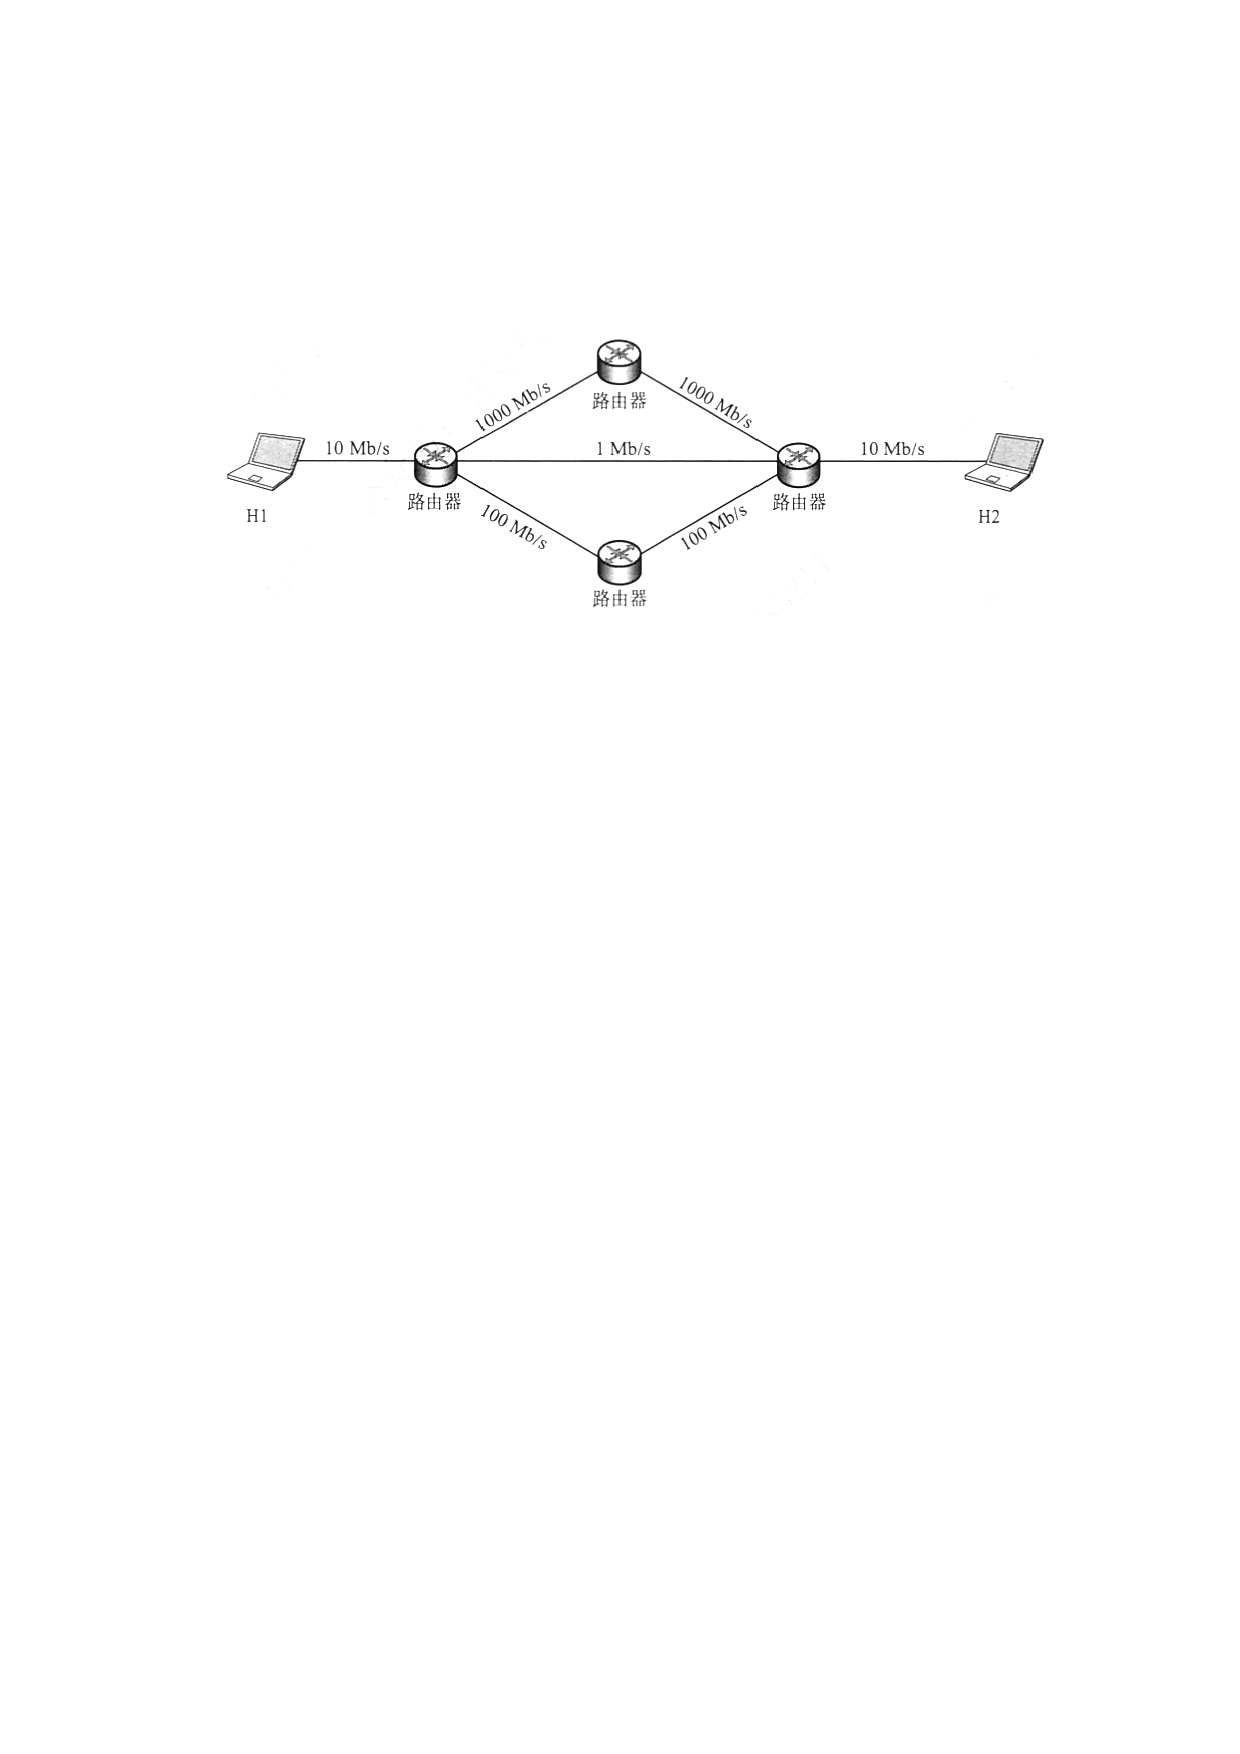
\includegraphics[width=.65\linewidth,height=.4\textheight,keepaspectratio]{../assets/figures/2024-questions-p004-b003.pdf}\end{center}

\begin{center}\begin{tabular}{>{\raggedright\arraybackslash}p{\dimexpr(\linewidth-8\tabcolsep)/4\relax}>{\raggedright\arraybackslash}p{\dimexpr(\linewidth-8\tabcolsep)/4\relax}>{\raggedright\arraybackslash}p{\dimexpr(\linewidth-8\tabcolsep)/4\relax}>{\raggedright\arraybackslash}p{\dimexpr(\linewidth-8\tabcolsep)/4\relax}}
\textbf{A.} 1Mb/s & \textbf{B.} 10Mb/s & \textbf{C.} 100Mb/s & \textbf{D.} 1 000Mb/s\\[.35em]\end{tabular}\end{center}

34．在下列二进制数字调制方法中，需要2 个不同频率载波的是\_\_\_\_\_\_。


\begin{center}\begin{tabular}{>{\raggedright\arraybackslash}p{\dimexpr(\linewidth-8\tabcolsep)/4\relax}>{\raggedright\arraybackslash}p{\dimexpr(\linewidth-8\tabcolsep)/4\relax}>{\raggedright\arraybackslash}p{\dimexpr(\linewidth-8\tabcolsep)/4\relax}>{\raggedright\arraybackslash}p{\dimexpr(\linewidth-8\tabcolsep)/4\relax}}
\textbf{A.} ASK & \textbf{B.} PSK & \textbf{C.} FSK & \textbf{D.} DPSK\\[.35em]\end{tabular}\end{center}

35．如题35 图所示的支持VLAN 划分的交换机，已按端口划分了3 个VLAN，部分端口连接主机的 IP 地址和MAC 地址如图中所示，ARP 表结构为<IP 地址，MAC 地址，TTL>。下列选项中，不 会出现在H4 的ARP 表中的是\_\_\_\_\_\_。 题35 图


\begin{center}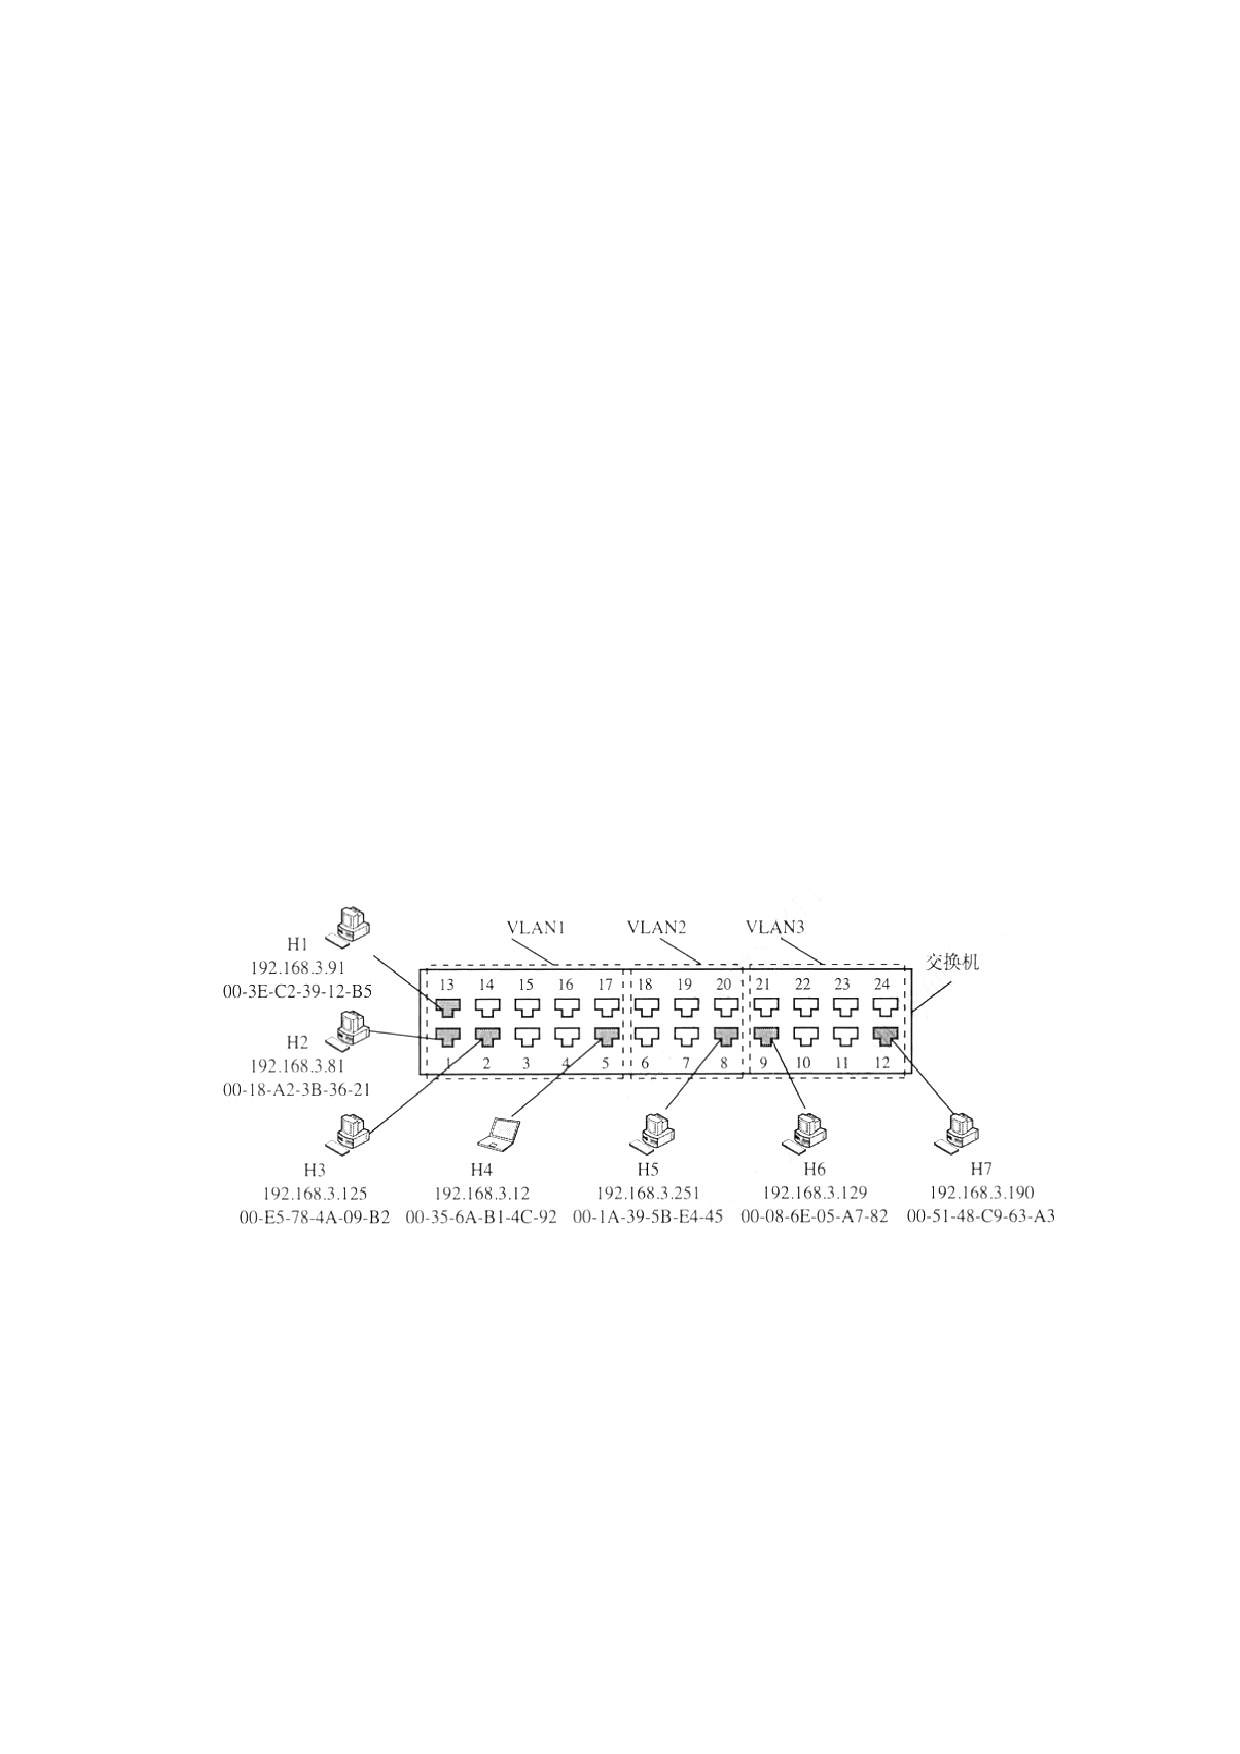
\includegraphics[width=.65\linewidth,height=.4\textheight,keepaspectratio]{../assets/figures/2024-questions-p004-b007.pdf}\end{center}

\begin{center}\begin{tabular}{>{\raggedright\arraybackslash}p{\dimexpr(\linewidth-4\tabcolsep)/2\relax}>{\raggedright\arraybackslash}p{\dimexpr(\linewidth-4\tabcolsep)/2\relax}}
\textbf{A.} 192.\allowbreak{}168.\allowbreak{}3.\allowbreak{}81, 00-18-A2-3B-36-21, 14:32:00 & \textbf{B.} 192.\allowbreak{}168.\allowbreak{}3.\allowbreak{}91, 00-3E-C2-39-12-B5, 14:37:00\\[.35em]
\textbf{C.} 192.\allowbreak{}168.\allowbreak{}3.\allowbreak{}125, 00-E5-78-4A-09-B2, 14:45:00 & \textbf{D.} 192.\allowbreak{}168.\allowbreak{}3.\allowbreak{}129, 00-08-6E-05-A7-82, 14:52:00\\[.35em]\end{tabular}\end{center}

36．在采用CSMA/CA 的802.11 无线局域网中，DIFS=128s，SIFS≥\(\displaystyle 28\,\mu\mathrm{s}\)，RTS、CTS 和ACK 帧的传输时延分别是\(\displaystyle 3\,\mu\mathrm{s}\)、2us 和\(\displaystyle 2\,\mu\mathrm{s}\)，忽略信号传播时延。若主机A 欲向AP 发送一个总长度为1 998B 的数据帧，无线链路带宽为54Mb/s，则隐藏站B 收到AP 发送的CTS 帧时，设置的网络分配向量 NAV 的值是\_\_\_\_\_\_。


\begin{center}\begin{tabular}{>{\raggedright\arraybackslash}p{\dimexpr(\linewidth-8\tabcolsep)/4\relax}>{\raggedright\arraybackslash}p{\dimexpr(\linewidth-8\tabcolsep)/4\relax}>{\raggedright\arraybackslash}p{\dimexpr(\linewidth-8\tabcolsep)/4\relax}>{\raggedright\arraybackslash}p{\dimexpr(\linewidth-8\tabcolsep)/4\relax}}
\textbf{A.} \(\displaystyle 326\,\mu\mathrm{s}\) & \textbf{B.} \(\displaystyle 354\,\mu\mathrm{s}\) & \textbf{C.} \(\displaystyle 385\,\mu\mathrm{s}\) & \textbf{D.} 51\(\displaystyle 3\,\mu\mathrm{s}\)\\[.35em]\end{tabular}\end{center}

37．主机甲通过选择重传（SR）滑动窗口协议向主机乙发送帧的部分过程如题37 图所示，\(\displaystyle F_x\) 为数据帧，\(\displaystyle ACK_x\) 为确认帧，x 是位数为3 比特的序号。乙只对正确接收的数据帧进行独立确认，发送窗口与接收窗口大小相同且均为最大值。甲在\(\displaystyle t_1\)时刻和\(\displaystyle t_2\)时刻发送的数据帧分别是\_\_\_\_\_\_。


第37题（续）：


\begin{center}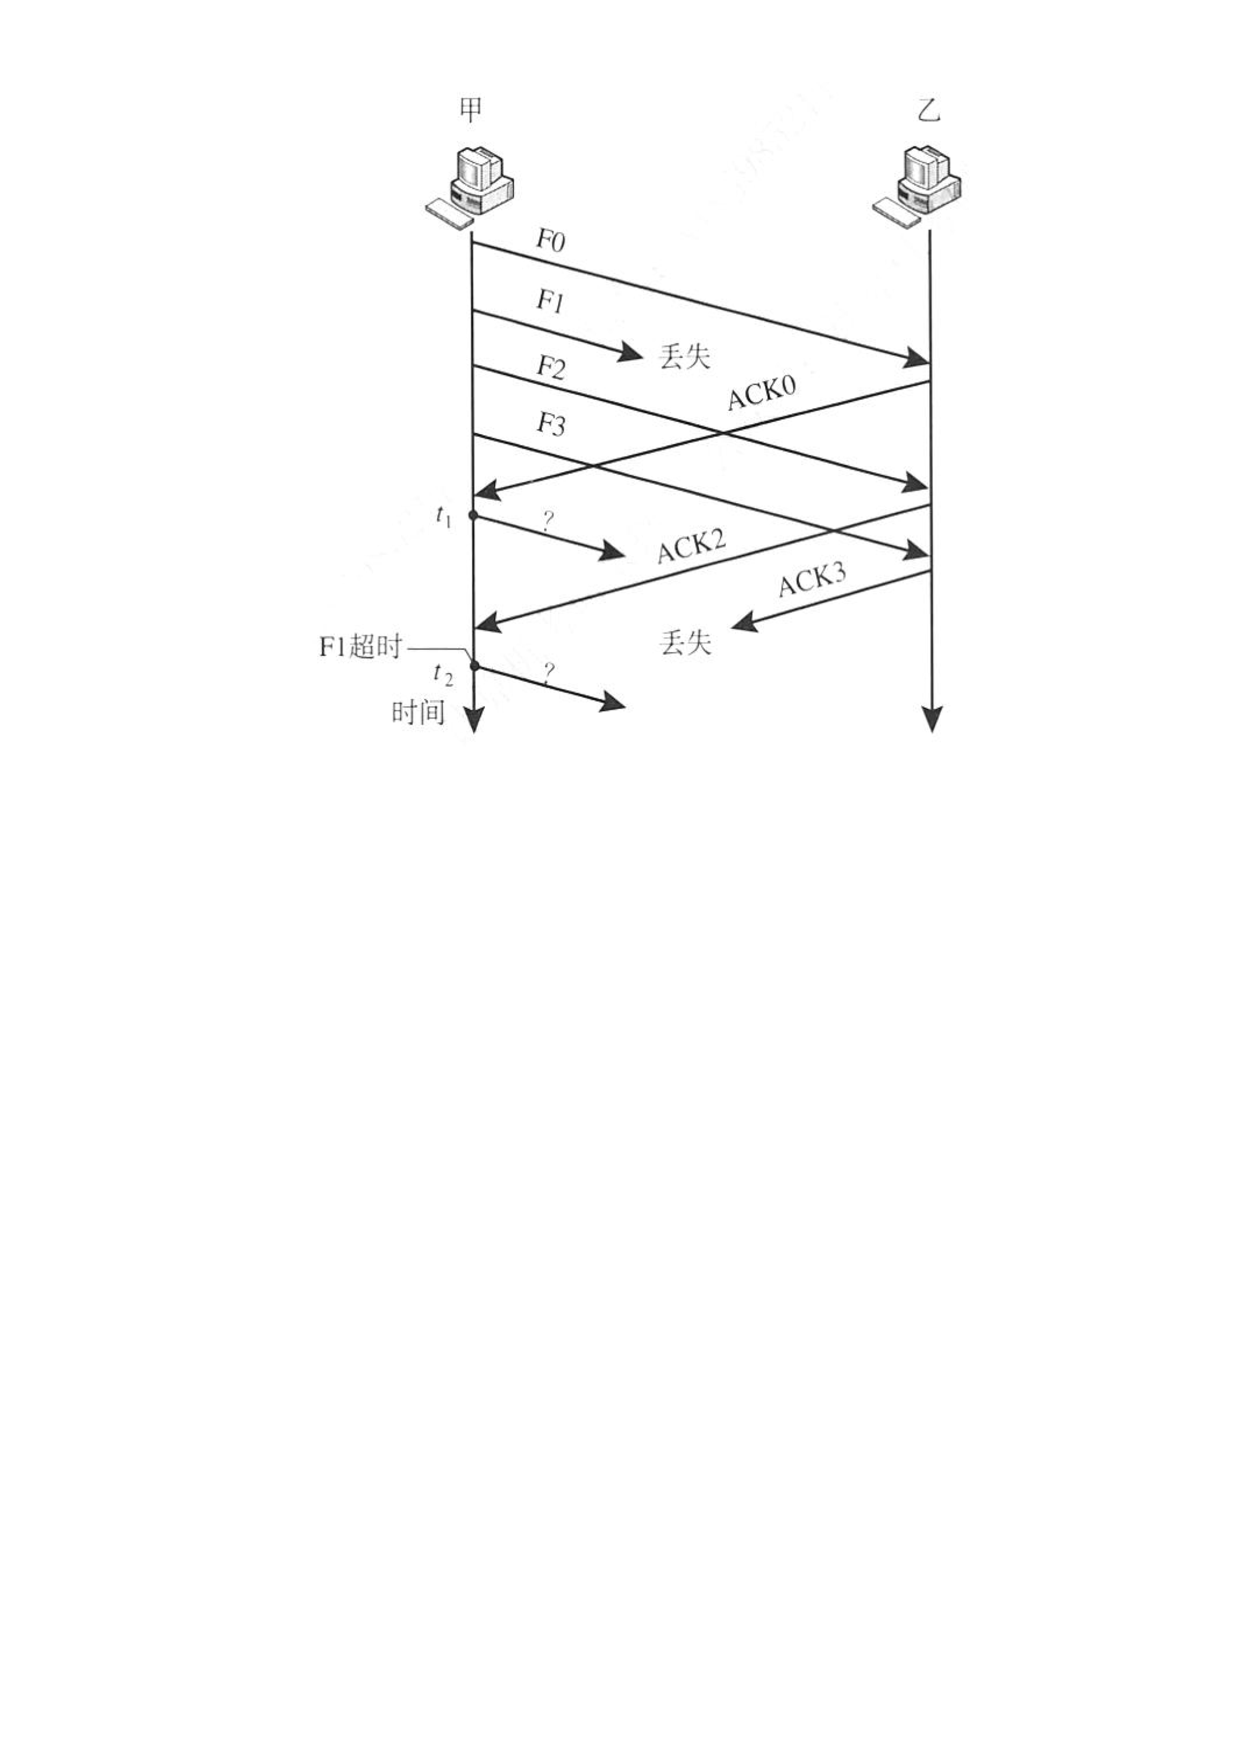
\includegraphics[width=.65\linewidth,height=.4\textheight,keepaspectratio]{../assets/figures/2024-questions-p005-b001.pdf}\end{center}

\begin{center}\begin{tabular}{>{\raggedright\arraybackslash}p{\dimexpr(\linewidth-8\tabcolsep)/4\relax}>{\raggedright\arraybackslash}p{\dimexpr(\linewidth-8\tabcolsep)/4\relax}>{\raggedright\arraybackslash}p{\dimexpr(\linewidth-8\tabcolsep)/4\relax}>{\raggedright\arraybackslash}p{\dimexpr(\linewidth-8\tabcolsep)/4\relax}}
\textbf{A.} F1, F3 & \textbf{B.} F1, F4 & \textbf{C.} F3, F1 & \textbf{D.} F4, F1\\[.35em]\end{tabular}\end{center}

38．假设主机H 通过TCP 向服务器发送长度为3000B 的报文，往返时间RTT=10ms，最长报文段寿命MSL=30s，最大报文段长度MSS=1 000B，忽略TCP 段的传输时延，报文传输结束后H 首先请求断开连接，则从H 请求建立TCP 连接时刻起，到H 进入CLOSED 状态为止，所需的时间至少是\_\_\_\_\_\_。


\begin{center}\begin{tabular}{>{\raggedright\arraybackslash}p{\dimexpr(\linewidth-8\tabcolsep)/4\relax}>{\raggedright\arraybackslash}p{\dimexpr(\linewidth-8\tabcolsep)/4\relax}>{\raggedright\arraybackslash}p{\dimexpr(\linewidth-8\tabcolsep)/4\relax}>{\raggedright\arraybackslash}p{\dimexpr(\linewidth-8\tabcolsep)/4\relax}}
\textbf{A.} 30.\allowbreak{}03s & \textbf{B.} 30.\allowbreak{}04s & \textbf{C.} 60.\allowbreak{}03s & \textbf{D.} 60.\allowbreak{}04s\\[.35em]\end{tabular}\end{center}

39．若UDP 协议在计算校验和过程中，计算得到中间结果为1011 1001 1011 0110 时，还需要加上最后一个16 位数0110 0101 1100 0101，则最终计算得到的校验和是\_\_\_\_\_\_。


\begin{center}\begin{tabular}{>{\raggedright\arraybackslash}p{\dimexpr(\linewidth-4\tabcolsep)/2\relax}>{\raggedright\arraybackslash}p{\dimexpr(\linewidth-4\tabcolsep)/2\relax}}
\textbf{A.} 0001 1111 0111 1011 & \textbf{B.} 0001 1111 0111 1100\\[.35em]
\textbf{C.} 1110 0000 1000 0011 & \textbf{D.} 1110 0000 1000 0100\\[.35em]\end{tabular}\end{center}

40．若浏览器不支持并行TCP 连接，使用非持久的HTTP/1.0 协议请求浏览1 个Web 页，该顶中引用同一网站上7 个小图像文件，则从浏览器为传输Web 页请求建立TCP 连接开始，到接收完所有内容为止，所需要的往返时间RTT 数至少是\_\_\_\_\_\_。


\begin{center}\begin{tabular}{>{\raggedright\arraybackslash}p{\dimexpr(\linewidth-8\tabcolsep)/4\relax}>{\raggedright\arraybackslash}p{\dimexpr(\linewidth-8\tabcolsep)/4\relax}>{\raggedright\arraybackslash}p{\dimexpr(\linewidth-8\tabcolsep)/4\relax}>{\raggedright\arraybackslash}p{\dimexpr(\linewidth-8\tabcolsep)/4\relax}}
\textbf{A.} 4 & \textbf{B.} 9 & \textbf{C.} 14 & \textbf{D.} 16\\[.35em]\end{tabular}\end{center}

\subsection*{二、综合应用题（第41～47小题，共70分）}

41．（13分）2023年10月26日，神舟十七号载人飞船发射取得圆满成功，再次彰显了中国航天事业的辉煌成就。载人航天工程是包含众多子工程的复杂系统工程，为了保证工程的有序开展，需要明确各子工程的前导子工程，以协调各子工程的实施。该问题可以简化、抽象为有向图的拓扑序列问题。已知有向图G采用邻接矩阵存储，类型定义如下。


\begin{Verbatim}[breaklines,breakanywhere,fontsize=\small]
typedef struct              // 图的类型定义
{
    int numVertices, numEdges;    // 图的顶点数和有向边数
    char VerticesList[MAXV];      // 顶点表，MAXV 为已定义常量
    int Edge[MAXV][MAXV];         // 邻接矩阵
}MGraph;
\end{Verbatim}

请设计算法：int uniquely(MGraph G)，判定G是否存在唯一的拓扑序列，若是，则返回1，否则返回0。要求如下。（1）给出算法的基本设计思想。（4分）（2）根据设计思想，采用C或C++语言描述算法，关键之处给出注释。（9分）


42．（10分）将关键字序列20, 3, 11, 18, 9, 14, 7依次存储到初始为空、长度为11的散列表HT中，散列函数\(\displaystyle H(\mathrm{key})=(\mathrm{key}\times3)\bmod11\)。\(\displaystyle H(\mathrm{key})\)计算出的初始散列地址为\(\displaystyle H_0\)，发生冲突时探查地址序列是\(\displaystyle H_1,\allowbreak H_2,\allowbreak H_3,\allowbreak \ldots\)，其中\(\displaystyle H_k=(H_0+k^2)\bmod11\)，\(\displaystyle k=1,\allowbreak 2,\allowbreak 3,\allowbreak \ldots\)。请回答下列问题。（1）画出所构造的HT，并计算HT的装填因子。（6分）（2）给出在HT中查找关键字14的关键字比较序列。（2分）（3）在HT中查找关键字8，确认查找失败时的散列地址是多少？（2分）


43．（13分）假定计算机M字长为32位，按字节编址，采用32位定长指令字，指令add、slli和lw的格式、编码和功能说明如题43图（a）所示。


\begin{center}\begin{adjustbox}{max width=\linewidth}\begin{tabular}{|>{\raggedright\arraybackslash}p{\dimexpr(\linewidth-14\tabcolsep-8\arrayrulewidth)/7\relax}|>{\raggedright\arraybackslash}p{\dimexpr(\linewidth-14\tabcolsep-8\arrayrulewidth)/7\relax}|>{\raggedright\arraybackslash}p{\dimexpr(\linewidth-14\tabcolsep-8\arrayrulewidth)/7\relax}|>{\raggedright\arraybackslash}p{\dimexpr(\linewidth-14\tabcolsep-8\arrayrulewidth)/7\relax}|>{\raggedright\arraybackslash}p{\dimexpr(\linewidth-14\tabcolsep-8\arrayrulewidth)/7\relax}|>{\raggedright\arraybackslash}p{\dimexpr(\linewidth-14\tabcolsep-8\arrayrulewidth)/7\relax}|>{\raggedright\arraybackslash}p{\dimexpr(\linewidth-14\tabcolsep-8\arrayrulewidth)/7\relax}|}\hline
指令 & 31–20 & 19–15 & 14–12 & 11–7 & 6–0 & 指令功能说明\\\hline
add & 0000000  rs2 & rs1 & 000 & rd & 0110011 & \(\displaystyle R[rd]\leftarrow R[rs1]+R[rs2]\)\\\hline
slli & 0000000  shamt & rs1 & 010 & rd & 0010011 & \(\displaystyle R[rd]\leftarrow R[rs1]\ll shamt\)\\\hline
lw & imm & rs1 & 010 & rd & 0000011 & \(\displaystyle R[rd]\leftarrow M[R[rs1]+imm]\)\\\hline\end{tabular}\end{adjustbox}\end{center}

其中，R[x]表示通用寄存器x的内容，M[x]表示地址为x的存储单元内容，shamt为移位位数，imm为补码表示的偏移量。题43图（b）给出了计算机M的部分数据通路及其控制信号（用带箭头虚线表示），其中，A和B分别表示从通用寄存器rs1和rs2中读出的内容；IR[31:20]表示指令寄存器中的高12位；控制信号Ext为0、1时扩展器分别实现零扩展、符号扩展，ALUctr为000、001、010时ALU分别实现加、减、逻辑左移运算。


\begin{center}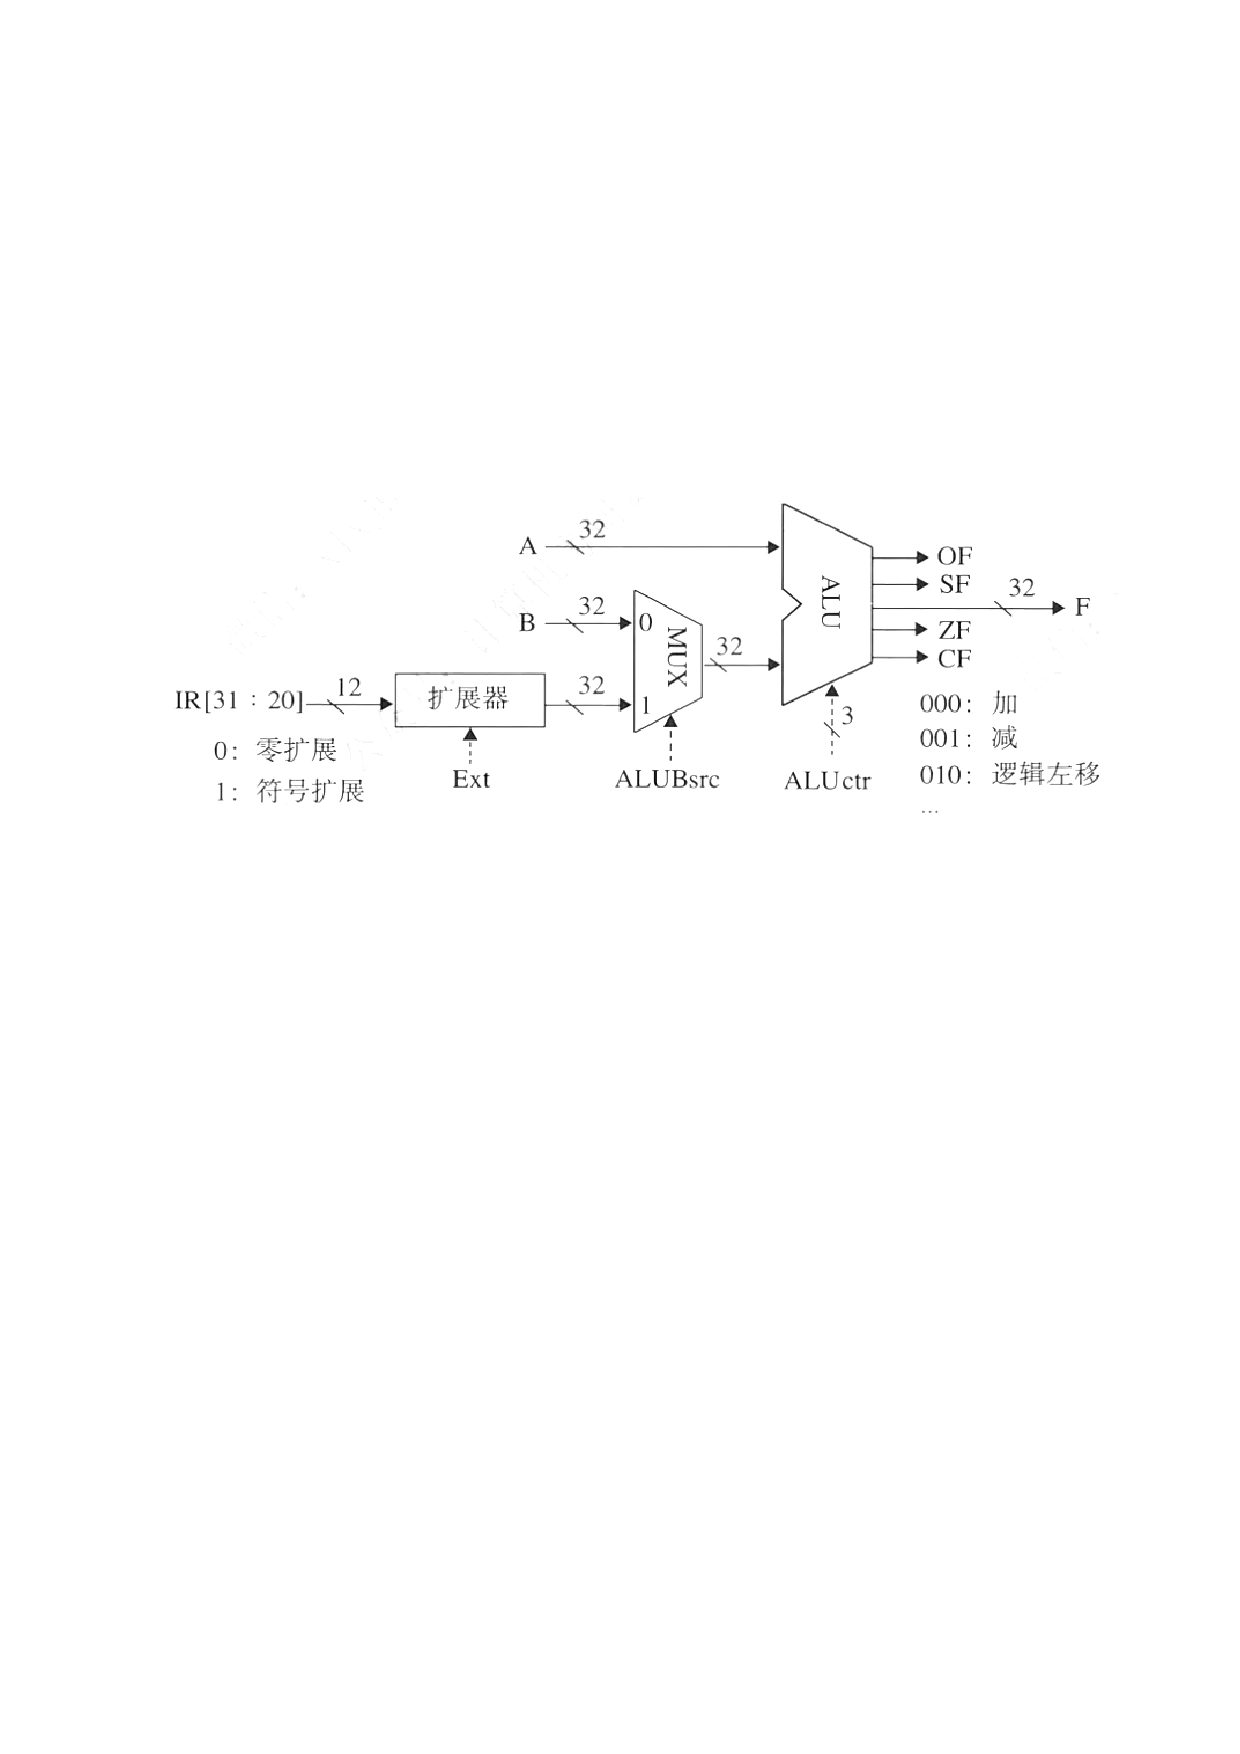
\includegraphics[width=.65\linewidth,height=.4\textheight,keepaspectratio]{../assets/figures/2024-questions-p008-b003.pdf}\end{center}

请回答下列问题。（1）计算机M最多有多少个通用寄存器？为什么shamt字段占5位？（2分）（2）执行add指令时，控制信号ALUBsrc的取值应是什么？若rs1和rs2寄存器内容分别是8765 4321H和9876 5432H，则add指令执行后，ALU输出端F、OF和CF的结果分别是什么？若该add指令处理的是无符号整数，则应根据哪个标志判断是否溢出？（5分）（3）执行slli指令时，控制信号Ext的取值可以是0也可以是1，为什么？（2分）（4）执行lw指令时，控制信号Ext、ALUctr的取值分别是什么？（2分）（5）若一条指令的机器码是A040 A103H，则该指令一定是lw指令，为什么？若执行该指令时，R[01H]=FFFF A2D0H，则所读取数据的存储地址是什么？（2分）


44．（10分）对于第43题中的计算机M，C语言程序P包含的语句“sum+=a[i];”在M中对应的指令序列S如下。


\begin{Verbatim}[breaklines,breakanywhere,fontsize=\small]
slli  r4, r2, 2       // R[r4]←R[r2]<<2
add   r4, r3, r4      // R[r4]←R[r3]+R[r4]
lw    r5, 0(r4)       // R[r5]←M[R[r4]+0]
add   r1, r1, r5      // R[r1]←R[r1]+R[r5]
\end{Verbatim}

已知变量i、sum和数组a都为int型，通用寄存器r1～r5的编号为01H～05H。请回答下列问题。（1）根据指令序列S中每条指令的功能，写出存放数组a的首地址、变量i和sum的通用寄存器编号。（3分）（2）已知M为小端方式计算机，采用页式存储管理方式，页大小为4KB。若执行到指令序列S中第1条指令时，i=5且r1和r3的内容分别为0000 1332H和0013 DFF0H，从地址0013 DFF0H开始的存储单元内容如题44图所示，则执行“sum+=a[i];”语句后，a[i]的地址、a[i]和sum的机器数分别是什么（用十六进制表示）？a[i]所在页的页号是多少？此次执行中，数组a至少存放在几页中？（5分）


\begin{center}\begin{adjustbox}{max width=\linewidth}\begin{tabular}{|c|c|c|c|c|c|c|c|c|}\hline
地址 & 0 & 1 & 2 & 3 & 4 & 5 & 6 & 7\\\hline
0013 DFF0 & FF & FF & FF & 7C & 70 & FE & FF & FF\\\hline
0013 DFF8 & 00 & 00 & 00 & 0C & 3C & 02 & 01 & FF\\\hline
0013 E000 & F0 & F1 & 00 & 00 & DC & EC & FF & FF\\\hline
0013 E008 & FF & FF & 01 & 02 & 00 & 00 & 01 & 02\\\hline\end{tabular}\end{adjustbox}\end{center}

（3）指令“slli r4, r2, 2”的机器码是什么（用十六进制表示）？若数组a改为short类型，则指令序列S中slli指令的汇编形式应是什么？（2分）


45．（7分）某计算机按字节编址，采用页式虚拟存储管理方式，虚拟地址和物理地址的长度均为32位，页表项的大小为4字节，页大小为4MB，虚拟地址结构如下。


\begin{center}\begin{adjustbox}{max width=\linewidth}\begin{tabular}{|>{\raggedright\arraybackslash}p{\dimexpr(\linewidth-4\tabcolsep-3\arrayrulewidth)/2\relax}|>{\raggedright\arraybackslash}p{\dimexpr(\linewidth-4\tabcolsep-3\arrayrulewidth)/2\relax}|}\hline
页号（10位） & 页内偏移量（22位）\\\hline\end{tabular}\end{adjustbox}\end{center}

进程P的页表起始虚拟地址为B8C0 0000H，被装载到从物理地址6540 0000H开始的连续主存空间中。请回答下列问题，要求答案用十六进制表示。（1）若CPU在执行进程P的过程中，访问虚拟地址1234 5678H时发生了缺页异常，经过缺页异常处理和MMU地址转换后得到的物理地址是BAB4 5678H，在此次缺页异常处理过程中，需要为所缺页分配页框并更新相应的页表项，则该页表项的虚拟地址和物理地址分别是什么？该页表项中的页框号更新后的值是什么？（3分）（2）进程P的页表所在页的页号是什么？该页对应的页表项的虚拟地址是什么？该页表项中的页框号是什么？（4分）


46．（8分）计算机系统中的进程之间往往需要相互协作以完成一个任务。在某网络系统中，缓冲区B用于存放一个数据分组，对B的操作有C1、C2和C3。C1将一个数据分组写入B中，C2从B中读出一个数据分组，C3对B中的数据分组进行修改。要求B为空时才能执行C1，B非空时才能执行C2和C3。（1）假设进程P1和P2均需要执行C1，实现C1的代码是否为临界区？为什么？（2分）（2）假设B初始为空，进程P1执行C1一次，进程P2执行C2一次。请定义尽可能少的信号量，并用wait()、signal()操作描述进程P1和P2之间的同步或互斥关系，说明所用信号量的作用及其初值。（3分）（3）假设B初始不为空，进程P1和P2各执行C3一次。请定义尽可能少的信号量，并用wait()、signal()操作描述进程P1和P2之间的同步或互斥关系，说明所用信号量的作用及其初值。（3分）


47．（9分）网络空间是继陆海空天之后的“第五疆域”，网络技术是网络疆域建设与治理的基础。路由算法与协议是网络核心技术之一，对其准确认知、合理选择与应用，对于网络建设十分重要。假设现有互联网中的4个自治系统互连拓扑示意图如题47图所示。其中，AS1运行内部网关协议RIP；AS3规模较小，自治系统内任意两个主机间通信，经过路由器数量不超过15个；AS4规模较大，自治系统内任意两个主机间通信，经过路由器数量可能超过20个。


\begin{center}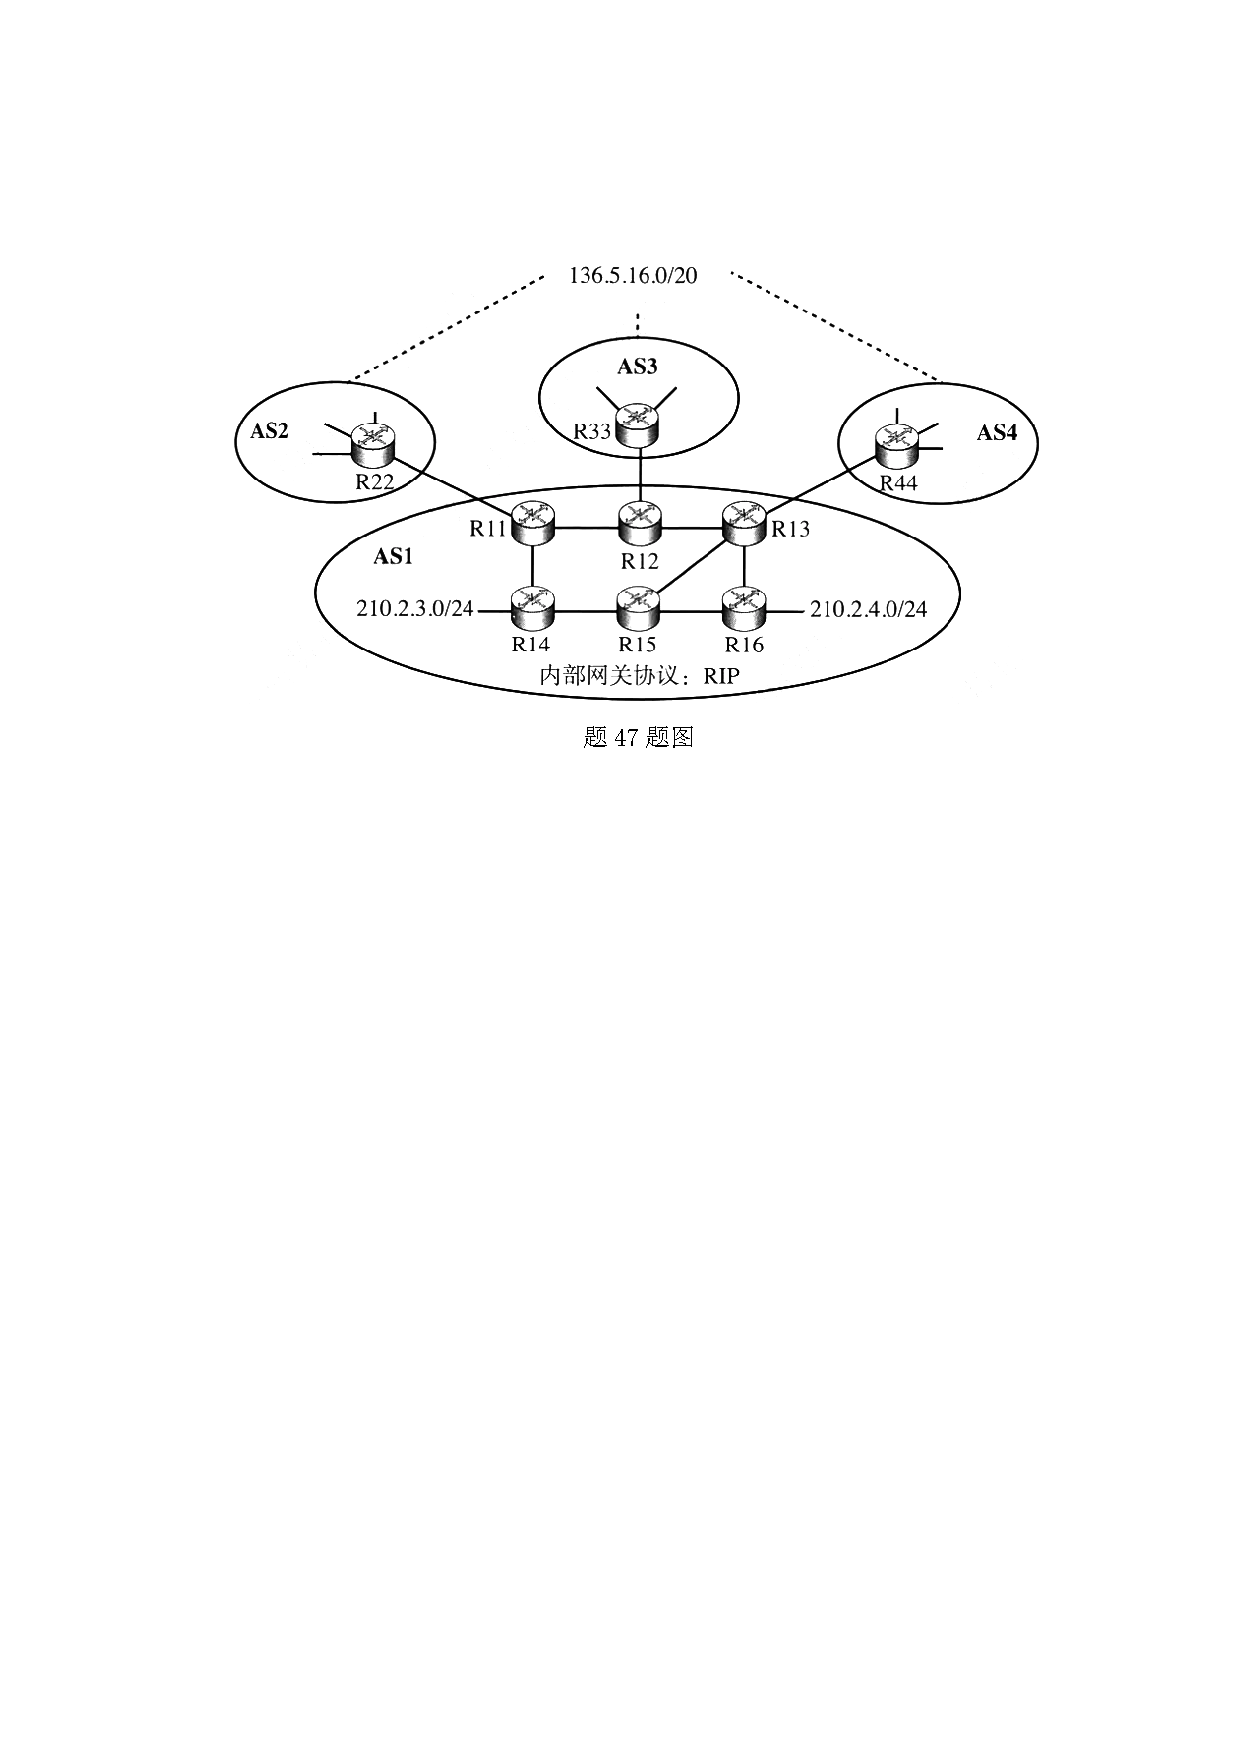
\includegraphics[width=.65\linewidth,height=.4\textheight,keepaspectratio]{../assets/figures/2024-questions-p012-b001.pdf}\end{center}

请回答下列问题。（1）若仅有RIP和OSPF内部网关协议供选择，则AS4应该选择哪个协议？（1分）（2）若AS3中的某主机向本自治系统内另一主机发送1个IP分组，为确保该IP分组能够被正常接收，则该IP分组的初始TTL值应该至少设置为多少？（1分）（3）假设AS1中的路由器同一时刻启动，启动后立即构建并交换初始距离向量，之后，每隔30s交换一次最新的距离向量，则从交换初始距离向量时刻算起，R11～R16路由器均获到达网络210.2.3.0/24的正确路由，至少需多长时间？均获到达网络210.2.4.0/24的正确路由，至少需多长时间？（2分）（4）R44向R13通告到达网络136.5.16.0/20路由时，由BGP协议哪类会话完成？通过哪个BGP报文通告？R13通过BGP协议的哪类会话将该网络可达性信息通告给R14和R15？（3分）（5）若R14和R15均收到分别由R11、R12、R13通告的到达网络136.5.16.0/20的可达性信息为：


\begin{center}\begin{adjustbox}{max width=\linewidth}\begin{tabular}{|>{\raggedright\arraybackslash}p{\dimexpr(\linewidth-6\tabcolsep-4\arrayrulewidth)/3\relax}|>{\raggedright\arraybackslash}p{\dimexpr(\linewidth-6\tabcolsep-4\arrayrulewidth)/3\relax}|>{\raggedright\arraybackslash}p{\dimexpr(\linewidth-6\tabcolsep-4\arrayrulewidth)/3\relax}|}\hline
目的网络 & AS路径 & 下一跳\\\hline
136.\allowbreak{}5.\allowbreak{}16.\allowbreak{}0/\allowbreak{}20 & AS2、AS8、AS19 & R11\\\hline
136.\allowbreak{}5.\allowbreak{}16.\allowbreak{}0/\allowbreak{}20 & AS3、AS7、AS11、AS19 & R12\\\hline
136.\allowbreak{}5.\allowbreak{}16.\allowbreak{}0/\allowbreak{}20 & AS4、AS10、AS19 & R13\\\hline\end{tabular}\end{adjustbox}\end{center}

则在无策略约束情况下，R14和R15更新路由表后，各自路由表中到达网络136.5.16.0/20路由的下一跳分别是什么（用路由器名称表示）？（2分）

\end{document}
